\documentclass[11pt,a4paper]{article}

\usepackage[margin=2.5cm]{geometry}
\usepackage{amsmath,amssymb}
\usepackage{booktabs}
\usepackage{graphicx}
\usepackage{xcolor}
\usepackage{siunitx}
\usepackage{hyperref}
\usepackage{cleveref}
\usepackage{enumitem}

\hypersetup{colorlinks=true,linkcolor=blue!70!black,citecolor=blue!70!black,urlcolor=blue!70!black}

\newcommand{\pb}{p_{\text{buy}}}
\newcommand{\ps}{p_{\text{sell}}}
\newcommand{\deltas}{\delta_s}
\newcommand{\netload}{d}
\newcommand{\Qb}{{Q^b}}
\newcommand{\Pb}{{P^b}}
\newcommand{\SoC}{{\text{SoC}^0}}
\newcommand{\ce}{\xi}
\newcommand{\ratio}[1]{R_{#1}}

% Observability ratio shorthand
\newcommand{\oratio}[1]{\frac{\theta^{\max}_{#1}-\theta^{\min}_{#1}}{|\theta^{\text{true}}_{#1}|}}

\title{Observability of Private Energy Data in Coalition Formation\\via Inverse Optimization}
\author{}
\date{}

\begin{document}
\maketitle

\begin{abstract}
We investigate the observability of agents' private data---consumption/generation profiles and battery characteristics---in a coalition formation framework for buildings with battery storage. An adversary observing only the broadcast net grid trades (and, in coalition, the internal exchange quantities) can reconstruct the set of private parameters consistent with the observed behaviour. We formulate the inverse problem as a linear program derived from the KKT conditions of the forward optimization, and compute per-parameter observability bounds for both singleton and coalition settings. Our results show that (i)~net load is partially observable from grid trades alone, with the battery creating significant ambiguity; (ii)~coalition participation \emph{increases} observability rather than decreasing it, because the coalition exchange vector reveals an additional equation per timestep; (iii)~the existing differential privacy mechanism protects the coalition structure but not the private data revealed through the ADMM broadcast.
\end{abstract}

% ===========================================================================
\section{Introduction}\label{sec:intro}
% ===========================================================================

Consider a set of $N$ buildings, each equipped with a battery storage system. At each MPC step $k$, every building solves a receding-horizon optimization over $h$ timesteps: minimise the cost of grid energy purchases (net of sales) subject to power balance, battery dynamics, and box constraints. The decision variables are the grid buy/sell quantities $g_{\text{buy}}[t], g_{\text{sell}}[t]$, the battery charge/discharge $\delta_s[t]$, and the state of charge $\text{SoC}[t]$.

\paragraph{Private parameters.}
Each building~$i$ has private data that it does not wish to reveal:
\begin{itemize}[nosep]
    \item \emph{Net load profile}: $\netload_i[t] = \text{cons}_i[t] - \text{prod}_i[t]$, the difference between predicted consumption and generation at each timestep.
    \item \emph{Battery capacity}: $\Qb_i$ (kWh).
    \item \emph{Battery power rating}: $\Pb_i$ (kW), the max charge/discharge rate.
    \item \emph{Initial state of charge}: $\SoC_i$ (kWh).
\end{itemize}

\paragraph{Public information.}
The following are known to all parties (including the adversary):
\begin{itemize}[nosep]
    \item Tariff: buy prices $\pb[t]$ and sell prices $\ps[t]$ for each timestep, with $\pb[t] > \ps[t]$.
    \item Battery efficiencies: $\eta_{\text{ch}} = \eta_{\text{dis}} = 0.95$ (uniform across all buildings; assumed known to the adversary).
\end{itemize}

\paragraph{Broadcast information.}
In the coalition formation framework (\texttt{privacy\_focussed\_coals}, \texttt{Coalition.jl:305}), each agent solves its MPC subproblem via ADMM and computes
\begin{equation}\label{eq:cons_vec}
    \text{cons\_vec}_i[t] = g_{\text{buy},i}[t] - g_{\text{sell},i}[t] \equiv z_i[t],
\end{equation}
the net grid trade at each timestep. This vector is shared with the coalition coordinator to evaluate pairwise coalition benefits (\texttt{Coalition.jl:360,369}). In a coalition of two or more agents, the ADMM consensus variable---the \emph{coalition exchange} $\ce_i[t]$---is also broadcast during iterations (\texttt{MPC\_optimiser.jl:269}).

\paragraph{Research question.}
Given the observed quantities $z_i^*[t]$ (and optionally $\ce_i^*[t]$), what is the set of private parameters $(\netload_i, \Qb_i, \Pb_i, \SoC_i)$ that could give rise to these observations? We call this the \emph{observability set}, and we quantify observability via per-parameter bounds.

% ===========================================================================
\section{Inverse Optimization Formulation}\label{sec:formulation}
% ===========================================================================

\subsection{Forward Problem}

The singleton MPC subproblem at step $k$ with horizon $h$ is the following LP:
\begin{subequations}\label{eq:forward}
\begin{align}
    \min_{g^+, g^-, \delta^+, \delta^-, c} \quad & \sum_{t=1}^{h} \bigl(\pb[t]\, g^+[t] - \ps[t]\, g^-[t]\bigr) \label{eq:obj}\\
    \text{s.t.} \quad & \netload[t] + g^-[t] + \delta^+[t] + \delta^-[t] = g^+[t] & \forall t \label{eq:power}\\
    & c[1] = \SoC \label{eq:init}\\
    & c[t] = c[t-1] + \eta_{\text{ch}}\,\delta^+[t-1] + \eta_{\text{ch}}^{-1}\,\delta^-[t-1] & \forall t \geq 2 \label{eq:dyn}\\
    & 0 \leq \delta^+[t] \leq \Pb, \quad -\Pb \leq \delta^-[t] \leq 0 & \forall t \label{eq:rate}\\
    & 0 \leq c[t] \leq \Qb & \forall t \label{eq:cap}\\
    & g^+[t] \geq 0, \quad g^-[t] \geq 0 & \forall t \\
    & \delta^+[h] + \delta^-[h] + c[h] \geq 0 \label{eq:final}
\end{align}
\end{subequations}
where $g^+, g^-$ are grid buy/sell, $\delta^+, \delta^-$ are charge/discharge, and $c$ is the SoC trajectory. The coalition LP adds a per-agent exchange variable $\ce_i[t]$ to the power balance~\eqref{eq:power} and a balance constraint $\sum_i \ce_i[t] = 0$.

\subsection{Inverse Problem}

Given an observation $z^*[t]$ (and optionally $\ce^*[t]$), the inverse problem finds all $(\theta, x, y)$---private parameters $\theta$, unobserved primal $x$, and dual variables $y$---satisfying:
\begin{enumerate}[nosep,label=(\roman*)]
    \item \emph{Primal feasibility}: \cref{eq:power}--\eqref{eq:final} (linear in $\theta$ and $x$).
    \item \emph{Observed trade}: $g^+[t] - g^-[t] = z^*[t]$ (linear).
    \item \emph{Strong duality}: $c'x = b'y$ (linear; LP strong duality is automatic).
    \item \emph{Complementary slackness}: constraints with nonzero duals are active (linear equalities).
\end{enumerate}
Since all conditions are linear, the inverse problem is itself an LP. For each private parameter $\theta_i$, we solve $\min \theta_i$ and $\max \theta_i$ over this LP to obtain the observability bounds $[\theta_i^{\min}, \theta_i^{\max}]$.

We define the \emph{observability ratio} for parameter $\theta_i$ as
\begin{equation}\label{eq:ratio}
    \ratio{i} = \frac{\theta_i^{\max} - \theta_i^{\min}}{|\theta_i^{\text{true}}|},
\end{equation}
where $\ratio{i} = 0$ means perfectly observable and large $\ratio{i}$ means highly ambiguous. The denominator uses $\max(|\theta_i^{\text{true}}|, 1)$ to avoid division by zero.

\paragraph{Two variants.}
We consider two levels of adversary knowledge:
\begin{itemize}[nosep]
    \item \emph{Feasibility-only} (Variant A): primal feasibility + observed trade only. What $\netload$ is consistent with $z^*$ and \emph{some} feasible battery operation?
    \item \emph{Optimality} (Variant B): full KKT conditions (strong duality + complementary slackness with duals from the forward solve). What $\netload$ is consistent with $z^*$ being \emph{optimal}?
\end{itemize}
Variant~B is tighter: the rationality assumption (the agent optimises) constrains the battery action, not just its feasibility. The full KKT derivation is given in \cref{app:kkt}.

\paragraph{Dual fixing.}
The strong duality constraint uses dual values $y^*$ extracted from the forward solve. This is a \emph{local} approximation: it is valid for perturbations of $\theta$ that do not change the active constraint set. For LPs, the dual is optimal over a neighbourhood of the primal optimum, so the bounds are valid but may not be tight (the true feasible set may be larger than the dual-fixed approximation suggests).

% ===========================================================================
\section{Singleton Results}\label{sec:singleton}
% ===========================================================================

We present results for building~1 ($\Qb = \SI{300}{kWh}$, $\Pb = \SI{75}{kW}$) at MPC step $k=20$ with horizon $h=16$, chosen to span a price change at $t=24$ ($\pb: 0.13 \to 0.17$). The battery is actively used for arbitrage, creating ambiguity in $\netload$.

\subsection{Per-Parameter Bounds}

\Cref{tab:singleton} shows the observability bounds for each private parameter, under both unknown and known battery assumptions.

\begin{table}[ht]
\centering
\caption{Singleton observability bounds for building~1 ($h=16$). ``Ratio'' is the observability ratio~\eqref{eq:ratio}; lower is more observable.}
\label{tab:singleton}
\small
\begin{tabular}{lr rr rr rr}
\toprule
& & \multicolumn{3}{c}{Battery unknown} & \multicolumn{3}{c}{Battery known} \\
\cmidrule(lr){3-5} \cmidrule(lr){6-8}
Param & True & Min & Max & Ratio & Min & Max & Ratio \\
\midrule
$\netload[1]$ & 55.3 & $-375.3$ & 124.8 & 9.04 & $-175.3$ & 124.7 & 5.42 \\
$\netload[6]$ & 55.6 & 2.0 & 502.1 & 9.00 & 2.0 & 77.1 & 1.35 \\
$\netload[14]$ & $-6.9$ & $-9.8$ & $-6.8$ & 0.43 & $-9.8$ & $-6.8$ & 0.43 \\
$\netload[16]$ & $-15.8$ & $-15.8$ & $-13.0$ & 0.17 & $-15.8$ & $-13.0$ & 0.17 \\
$\Qb$ & 300 & 0 & 2000 & 6.67 & \multicolumn{3}{c}{(known)} \\
$\Pb$ & 75 & 0 & 500 & 6.67 & \multicolumn{3}{c}{(known)} \\
$\SoC$ & 0 & 0 & 0.07 & 0.07 & \multicolumn{3}{c}{(known)} \\
\bottomrule
\end{tabular}
\end{table}

Key observations:
\begin{itemize}[nosep]
    \item \emph{$\netload$ is tightly observable when the battery hits limits.} At $t=14$--$16$, the battery is empty (final constraint active), so $\deltas \approx 0$ and $\netload \approx z^*$. The ratio drops to $\sim 0.2$.
    \item \emph{During active arbitrage, $\netload$ is wide.} At $t=1$--$8$, the battery charges/discharges, and $\deltas$ is a free variable (within box constraints). The ratio is $\sim 9$.
    \item \emph{$\Qb$ and $\Pb$ are unobservable.} Their bounds span the full prior range. The battery's capacity and power rating are never directly revealed by the grid trade---only their \emph{effect} (via the feasible $\deltas$ trajectory) is visible.
    \item \emph{Knowing the battery helps.} With known $\Qb, \Pb, \SoC$, the mean $\netload$ ratio drops from 11.1 to 3.0 (\cref{fig:cross_building}).
\end{itemize}

\subsection{Cross-Building Comparison}

\Cref{fig:cross_building} compares observability across buildings with different battery sizes.

\begin{figure}[ht]
    \centering
    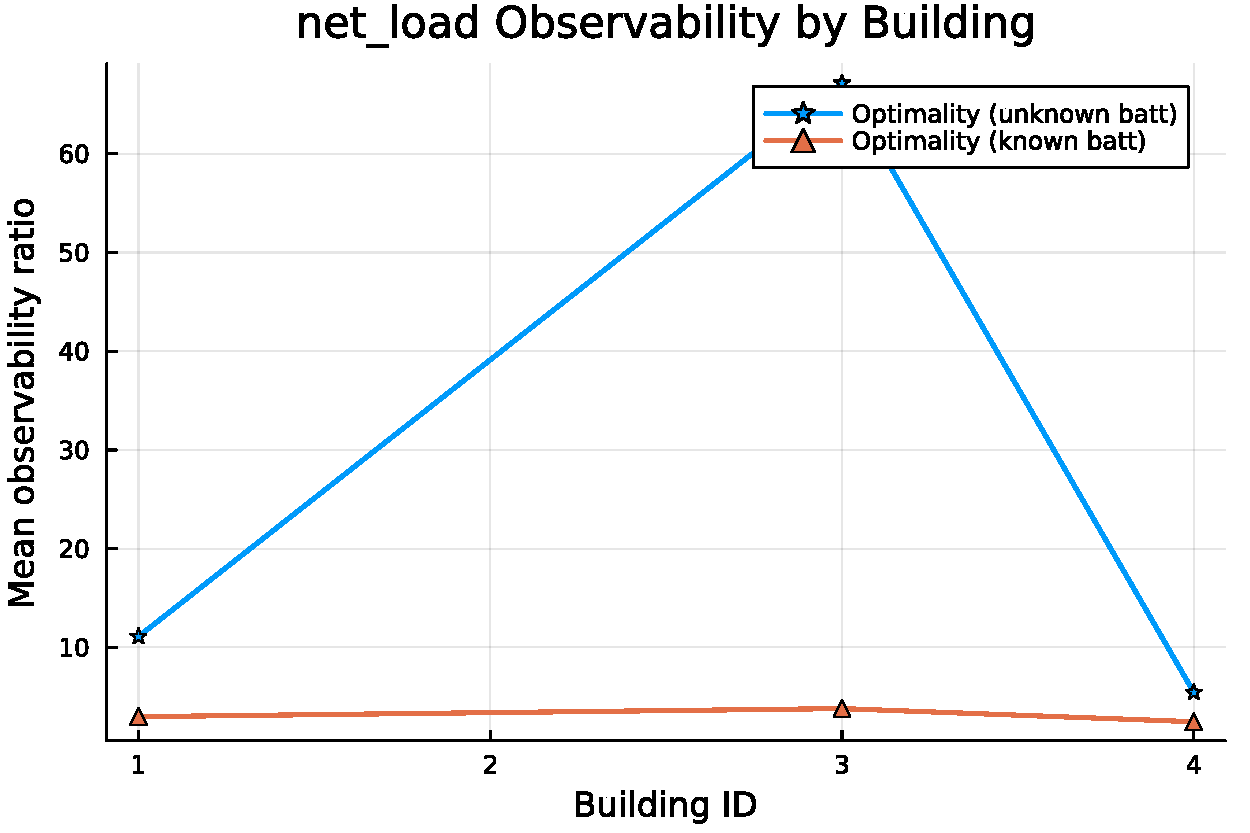
\includegraphics[width=0.8\textwidth]{figs/cross_building.pdf}
    \caption{Mean $\netload$ observability ratio for three buildings with different battery sizes. Building~3 ($\Qb=50$, small battery) is hardest to observe; building~4 ($\Qb=500$, large battery) is easiest. Knowing the battery parameters (dashed) roughly halves the ratio for all buildings.}
    \label{fig:cross_building}
\end{figure}

The counterintuitive result that larger batteries \emph{improve} observability arises because large batteries hit their capacity limits more often, creating binding constraints that pin $\deltas$ and hence $\netload$.

\subsection{Horizon Sensitivity}

\Cref{fig:horizon} shows how observability scales with the horizon length $h$.

\begin{figure}[ht]
    \centering
    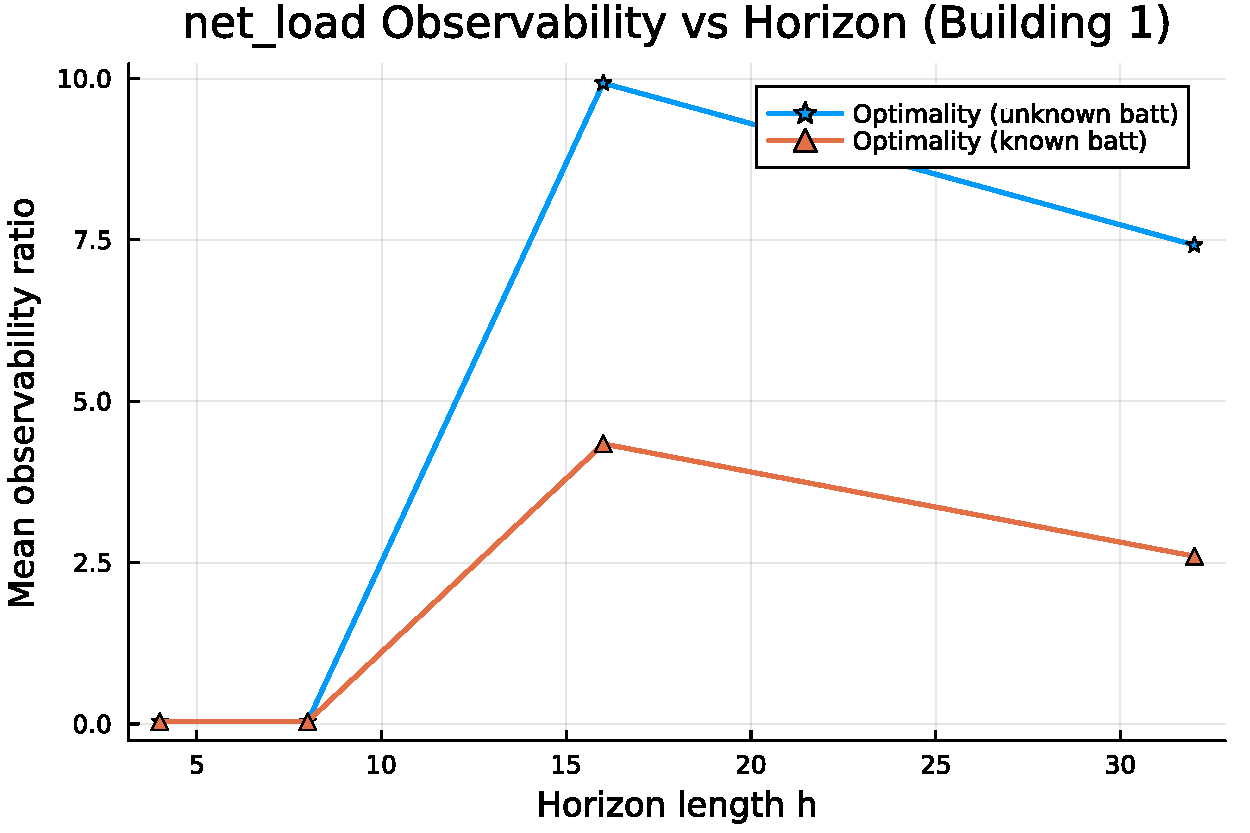
\includegraphics[width=0.8\textwidth]{figs/horizon.pdf}
    \caption{$\netload$ observability ratio vs.\ horizon length for building~1. Short horizons ($h \leq 8$) have no price variation, so the battery is unused and $\netload = z^*$ (trivially observable). At $h=16$, the price change activates the battery and observability degrades sharply. Longer horizons ($h=32$) provide more data, slightly improving observability.}
    \label{fig:horizon}
\end{figure}

% ===========================================================================
\section{Coalition Results}\label{sec:coalition}
% ===========================================================================

We now consider a 2-agent coalition (buildings~1 and~3) at the same MPC step $k=20$, $h=16$. The coalition is solved both centrally (LP with $\sum_i \ce_i = 0$) and via ADMM (per-agent QP subproblems with a quadratic consensus penalty).

\subsection{Three Observation Models}

\begin{table}[ht]
\centering
\caption{Coalition observability: mean $\netload$ ratio across all $h=16$ timesteps. Lower is more observable. Battery parameters are assumed known.}
\label{tab:coalition}
\small
\begin{tabular}{lc rr}
\toprule
Model & Observation & Agent~1 & Agent~2 \\
\midrule
A (converged, $z^*$ only) & $z_i^*$ & 80.96 & 268.33 \\
B (converged, $z^* + \ce^*$) & $z_i^*,\ \ce_i^*$ & \textbf{1.64} & \textbf{1.27} \\
C (trajectory, 5 iters) & $z_i^{(j)},\ \ce_i^{(j)},\ \forall j$ & 2.65 & 2.06 \\
C (trajectory, 10 iters) & $z_i^{(j)},\ \ce_i^{(j)},\ \forall j$ & 2.65 & 2.05 \\
C (trajectory, 20 iters) & $z_i^{(j)},\ \ce_i^{(j)},\ \forall j$ & 2.63 & 2.05 \\
\bottomrule
\end{tabular}
\end{table}

\paragraph{Model A ($z^*$ only): unobservable.}
Without observing $\ce_i^*$, the coalition exchange is a free variable. The other agent's $\ce$ can absorb any discrepancy in $\netload$, so the bounds hit the prior limits ($\ratio{} \approx 80$--$268$). This is the same as the singleton case with unknown battery: the free variables swamp the signal.

\paragraph{Model B ($z^* + \ce^*$): tightest.}
Observing both the converged grid trade and the coalition exchange gives $\ratio{} \approx 1.3$--$1.6$. The power balance $\netload + \deltas + \ce^* = z^* - g^-[t]$ provides one equation per timestep with $\ce^*$ known, reducing the ambiguity to the battery action $\deltas$ alone. With known battery parameters and strong duality (which pins $\deltas$ via optimality), the bounds are tight.

\paragraph{Model C (ADMM trajectory): intermediate.}
Each ADMM iteration~$j$ solves a QP:
\begin{equation}
    \min \sum_t \bigl(\pb\, g^{+,(j)} - \ps\, g^{-,(j)}\bigr) + \lambda^{(j)\prime} \ce^{(j)} + \frac{c}{2}\|\ce^{(j)} - \text{ct}^{(j)}\|^2.
\end{equation}
The ADMM subproblem is a convex QP, but the only quadratic term involves $\ce$, which is observed. At the observed optimum, the stationarity condition for the free variable $\ce$ is satisfied ($\mu = \lambda + c(\ce_j - \text{ct})$), so the $Q^+$ term in the dual vanishes. With $\ce$ fixed to $\ce^{(j)}$, the quadratic term in the objective is a known constant $K^{(j)}$, and all KKT conditions---including strong duality---are linear in the private parameters. The inverse problem is therefore an LP. (If $\ce$ were not observed, the strong duality would contain a quadratic term in $\ce$, making the inverse problem a QCQP.) LP strong duality gives a linear equation in $\netload$ with the per-iteration dual $\mu^{(j)}$ (extracted from the subproblem). Multiple iterations provide multiple equations, but the duals barely change across iterations (the active set is determined by the tariff, not the ADMM parameters), so the tightening is modest: $\ratio{} \approx 2.1$--$2.7$.

The trajectory model is wider than Model~B because (i)~complementary slackness is disabled across iterations (SCS dual noise at $10^{-4}$ tolerance makes exact CS constraints infeasible when stacked), and (ii)~the strong duality tolerance must be widened ($\pm 0.5$) to accommodate the SCS duality gap.

\begin{figure}[ht]
    \centering
    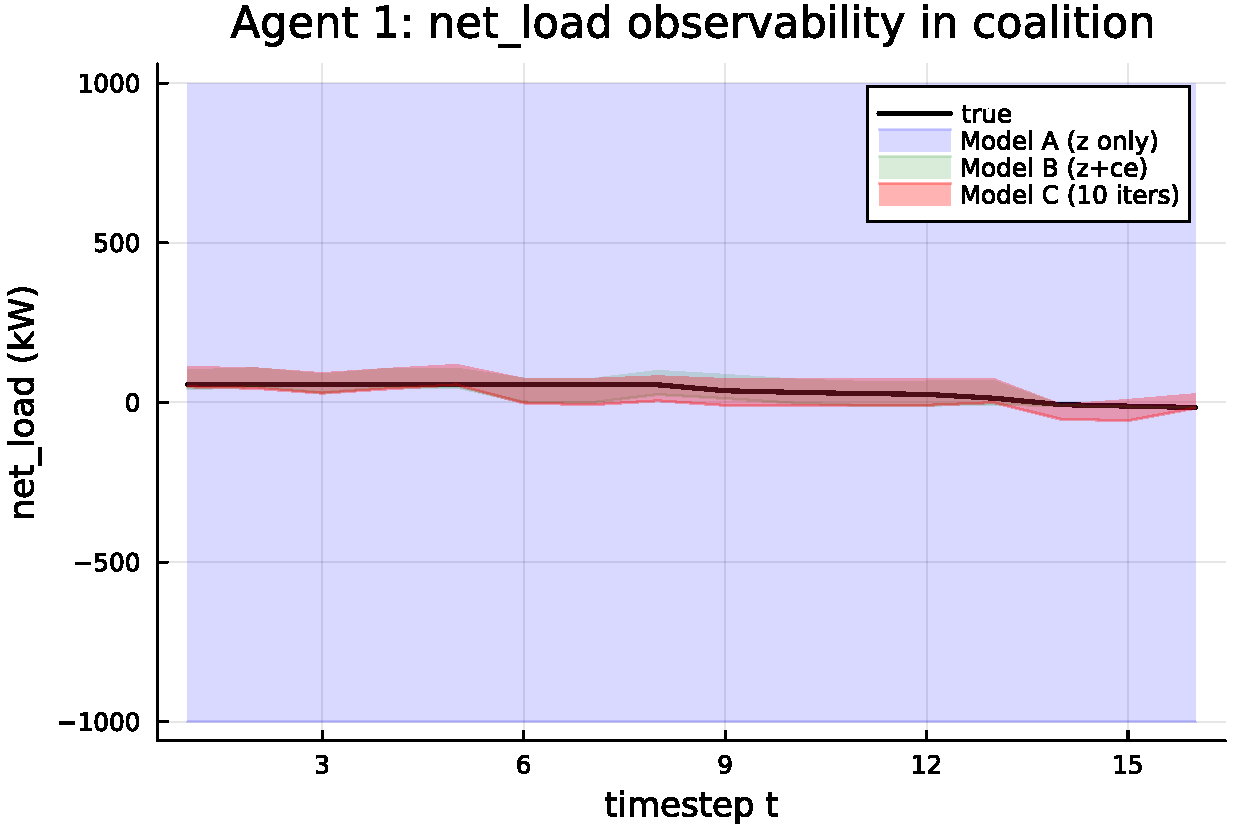
\includegraphics[width=0.8\textwidth]{figs/coal_bounds.pdf}
    \caption{Per-timestep $\netload$ bounds for agent~1 in the 2-agent coalition. Model~A (blue) is unbounded; Model~B (green) is tightest; Model~C with 10 iterations (red) is intermediate. The true $\netload$ (black) lies within all bounds.}
    \label{fig:coal_bounds}
\end{figure}

% ===========================================================================
\section{Comparison: Singleton vs.\ Coalition}\label{sec:comparison}
% ===========================================================================

\Cref{tab:comparison} compares the singleton and coalition settings (both with known battery).

\begin{table}[ht]
\centering
\caption{Mean $\netload$ observability ratio: singleton vs.\ coalition (known battery, $h=16$).}
\label{tab:comparison}
\small
\begin{tabular}{l r r}
\toprule
Setting & Agent~1 (Bldg~1) & Agent~2 (Bldg~3) \\
\midrule
Singleton & 3.0 & 3.8 \\
Coalition, Model~B ($z^* + \ce^*$) & \textbf{1.6} & \textbf{1.3} \\
Coalition, Model~C (trajectory) & 2.7 & 2.1 \\
\bottomrule
\end{tabular}
\end{table}

\paragraph{Coalition participation increases observability.}
This is the central finding. In the singleton case, the adversary observes $z^* = \netload + \deltas$ and must disentangle $\netload$ from the battery action $\deltas$. In the coalition case (Model~B), the adversary observes $z^*$ \emph{and} $\ce^*$, and the power balance gives $\netload = (z^* - \ce^*) - \deltas$. While $\deltas$ is still unknown, the coalition exchange $\ce^*$ provides additional structure: it is the result of an optimisation that balances both agents' net loads, and the strong duality constraint (with duals from the centralised LP) pins the battery trajectory more tightly.

Intuitively, the coalition exchange $\ce^*$ reveals information about the \emph{difference} between the agents' net loads (agents trade when one has surplus and the other has deficit). This structural information constrains $\netload$ beyond what the grid trade alone provides.

% ===========================================================================
\section{Differential Privacy and \texorpdfstring{$\delta_G$}{delta\_G} Scaling}\label{sec:dp}
% ===========================================================================

\subsection{The Exponential Mechanism}

The coalition formation algorithm (\texttt{privacy\_focussed\_coals\_with\_delta}, \texttt{Coalition.jl:305}) uses an exponential mechanism to select which agent pairs form coalitions. The utility of a pair $(i,j)$ is the coalition benefit:
\begin{equation}
    u(i,j) = \sum_t \bigl(\pb[t] - \ps[t]\bigr) \cdot \min\bigl(|z_i[t]|,\ |z_j[t]|\bigr) \cdot \mathbb{1}[z_i[t] \cdot z_j[t] < 0],
\end{equation}
computed from the broadcast cons\_vec (i.e., $z_i$). The sensitivity is bounded by
\begin{equation}
    \Delta_u = \delta_G \cdot \max_t |\pb[t] - \ps[t]| = \delta_G \cdot 0.10,
\end{equation}
where $\delta_G$ is a scaling parameter. The sampling weights are
\begin{equation}\label{eq:softmax}
    w(i,j) \propto \exp\!\left(\frac{\epsilon \cdot u(i,j)}{2\,\Delta_u}\right), \quad \epsilon = 1.
\end{equation}

\subsection{What Is Protected}

The exponential mechanism provides $\epsilon$-differential privacy for the \emph{coalition structure}: which agents are paired together. The post-processing theorem guarantees that any function of the (randomised) coalition structure is also $\epsilon$-DP.

\subsection{What Is Not Protected}

Crucially, the DP mechanism does \emph{not} protect the data used to compute the utility:
\begin{enumerate}[nosep]
    \item \textbf{The net grid trade $z_i^*$} (cons\_vec) is computed from the ADMM solve and shared with the coordinator \emph{before} the exponential mechanism is applied (\texttt{Coalition.jl:360}). This is the very quantity our inverse optimisation uses.
    \item \textbf{The coalition exchange $\ce_i^*$} is broadcast during ADMM iterations (\texttt{MPC\_optimiser.jl:269}). In Model~B, this provides the tightest bounds.
    \item \textbf{The private parameters} $(\netload, \Qb, \Pb, \SoC)$ are inferable from the above via inverse optimisation, as demonstrated in \cref{sec:singleton,sec:coalition}.
\end{enumerate}

The post-processing theorem does not apply because the ADMM solve is \emph{not} a post-processing of the coalition structure: it uses the private data directly. The DP guarantee covers the \emph{selection} of coalitions, not the \emph{computation within} a formed coalition.

\subsection{Scaling with $\delta_G$}

The parameter $\delta_G$ controls the privacy--utility trade-off of the coalition selection:

\begin{description}[nosep]
    \item[$\delta_G \to 0$ (deterministic):] $\Delta_u \to 0$ and the softmax~\eqref{eq:softmax} degenerates to argmax. The coalition structure is fully revealed (no privacy), but the utility is maximised. The adversary learns which pairs have the highest benefit---but $z_i^*$ is already shared, so the private parameters are equally observable regardless.
    \item[$\delta_G \to \infty$ (uniform):] $\Delta_u \to \infty$ and the softmax becomes uniform. The coalition structure is fully randomised ($\epsilon$-DP), but the adversary still observes $z_i^*$ and $\ce_i^*$, and can infer the private parameters just as well.
\end{description}

In both extremes, the observability of private parameters from the broadcast data is \emph{unchanged}. The $\delta_G$ parameter trades off coalition-structure privacy against coalition quality; it does \emph{not} affect the information leakage through the optimisation broadcasts.

This is a fundamental gap in the privacy guarantee: the exponential mechanism randomises the \emph{output} of the coalition selection, but the \emph{inputs} (net grid trades, coalition exchanges) are transmitted in the clear. Closing this gap requires either (i)~adding noise to the broadcast $z_i^*$ itself (at the cost of coalition quality), or (ii)~using secure multiparty computation to compute the coalition benefit without revealing individual $z_i$ values.

\subsection{Empirical \texorpdfstring{$\delta_G$}{delta\_G} Sweep}

\Cref{fig:sweep} shows an empirical sweep over $\delta_G \in [0, 10^4]$ for 10 buildings (day~37, 10 repeats per point). The four panels show average cost, cost std, execution time, and ADMM iterations as $\delta_G$ varies.

\begin{figure}[ht]
    \centering
    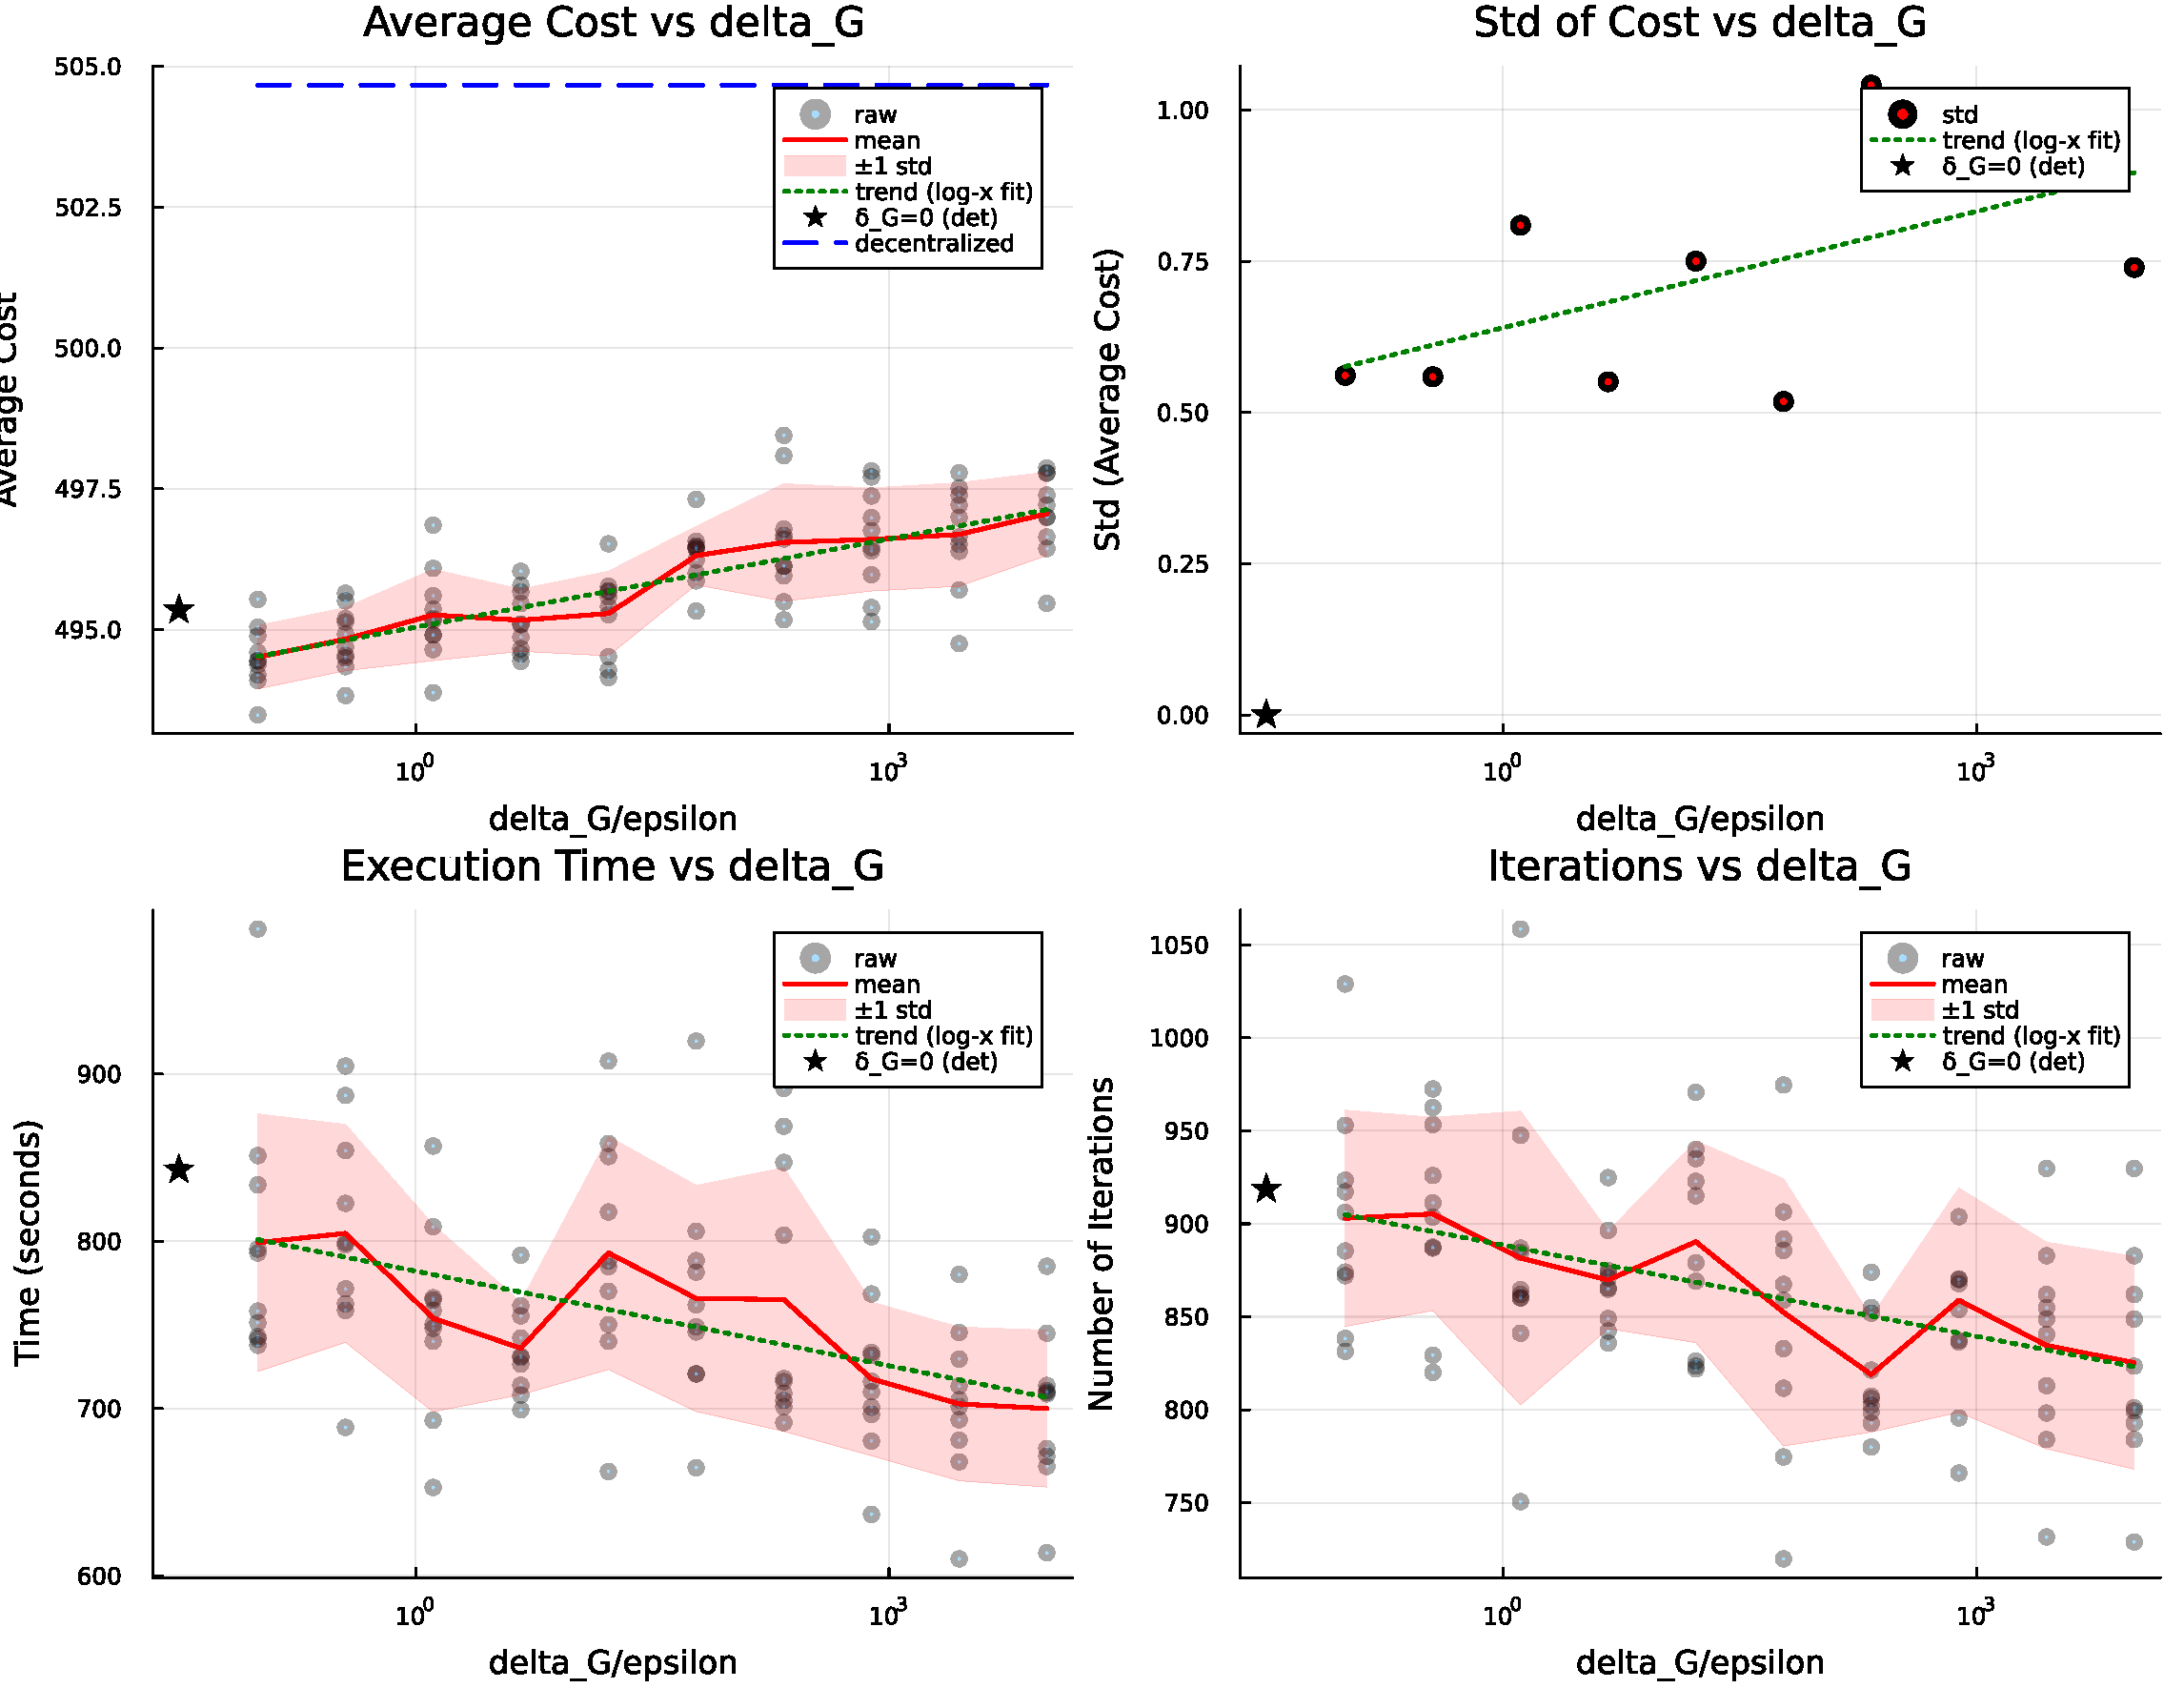
\includegraphics[width=\textwidth]{figs/sweep.pdf}
    \caption{Sweep over $\delta_G$ for 10 buildings (day~37, 10 repeats per point). \emph{Top-left:} average cost per building (dashed = decentralised baseline). \emph{Top-right:} std of cost across repeats. \emph{Bottom-left:} execution time. \emph{Bottom-right:} ADMM iterations per MPC step. The $\delta_G=0$ anchor (star) is deterministic (std=0).}
    \label{fig:sweep}
\end{figure}

The decentralised baseline cost is 504.67; the deterministic coalition ($\delta_G=0$) achieves 495.35---a benefit of 1.84\%. At $\delta_G=0.1$ (near-greedy), the benefit rises slightly to 2.01\% with std 0.56. At $\delta_G=10^4$ (near-uniform), the benefit drops to 1.51\% with std 0.74. The cost is remarkably flat across the entire range: the coalition benefit varies by only $\sim$0.5 percentage points.

Two observations are relevant for privacy:

\begin{enumerate}[nosep]
    \item \emph{The privacy--utility tradeoff is mild.} Randomising the coalition structure (large $\delta_G$) degrades the coalition benefit by only $\sim$0.5pp relative to the deterministic optimum. The exponential mechanism provides strong coalition-structure privacy at minimal cost.
    \item \emph{Observability is independent of $\delta_G$.} Regardless of which coalitions form, each agent's $z_i^*$ is broadcast to the coordinator for the pair-compatibility check (\texttt{Coalition.jl:360}), and $\ce_i^*$ is broadcast during ADMM. The inverse optimisation uses these broadcasts, not the coalition structure. The observability bounds in \cref{sec:singleton,sec:coalition} are therefore unchanged by $\delta_G$: the adversary infers the private parameters equally well at $\delta_G=0$ and $\delta_G=10^4$.
\end{enumerate}

This confirms the fundamental gap identified above: the $\delta_G$ parameter trades off coalition-structure privacy against coalition quality, \emph{not} data privacy against coalition quality. The data is always revealed through the optimisation broadcasts.

% ===========================================================================
\section{Conclusions}\label{sec:conclusions}
% ===========================================================================

We have shown that an adversary observing the broadcast grid trades and coalition exchanges can reconstruct the set of private parameters consistent with the observed behaviour, formulated as a linear program derived from the KKT conditions. The key findings are:

\begin{enumerate}[nosep]
    \item Net load is partially observable from grid trades alone (ratio $\sim 9$ with unknown battery, $\sim 3$--$5$ with known battery), with the battery creating significant ambiguity during active arbitrage.
    \item Battery parameters ($\Qb, \Pb$) are essentially unobservable from grid trades alone.
    \item Coalition participation \emph{increases} observability (ratio drops from $\sim 3$ to $\sim 1.3$--$1.6$) because the coalition exchange $\ce^*$ reveals additional structural information.
    \item The existing DP mechanism protects the coalition structure but not the private data revealed through the ADMM broadcasts. The $\delta_G$ parameter has no effect on the observability of private parameters.
\end{enumerate}

Future work should explore noise injection on the broadcast quantities (differential privacy on $z_i^*$ and $\ce_i^*$ directly), or secure multiparty computation protocols that avoid revealing individual agents' trades to the coordinator.

% ===========================================================================
\appendix
\section{KKT Derivation for the Inverse LP}\label{app:kkt}
% ===========================================================================

\subsection{Lagrangian}

The forward LP~\eqref{eq:forward} has equality constraints (power balance, battery dynamics, initial SoC) and inequality constraints (box bounds, final constraint). The Lagrangian is:
\begin{equation}
    L = \sum_t \bigl(\pb\, g^+ - \ps\, g^-\bigr) - \sum_t \mu_t \bigl(\netload + g^- + \delta^+ + \delta^- - g^+\bigr) - \lambda_0 \bigl(c[1] - \SoC\bigr) - \sum_{t \geq 2} \lambda_t \bigl(c[t] - c[t-1] - \eta_{\text{ch}} \delta^+[t-1] - \eta_{\text{ch}}^{-1} \delta^-[t-1]\bigr).
\end{equation}

\subsection{Stationarity}

Setting $\partial L / \partial g^+ = 0$: $\pb - \mu \leq 0$, i.e.\ $\mu \geq \pb$. But SCS returns $-\mu$ for equality constraints, so in practice $-\mu \in [\ps, \pb]$, giving $\ps \leq -\mu \leq \pb$.

Setting $\partial L / \partial g^- = 0$: $-\ps + \mu \leq 0$, i.e.\ $\mu \leq \ps$.

Combining: $\ps \leq -\mu \leq \pb$ (the net grid price lies between buy and sell).

Setting $\partial L / \partial \delta^+ = 0$: the reduced cost is $\mu - \eta_{\text{ch}} \lambda_{t+1}$, bounded by the dual of the upper bound $\alpha_t \geq 0$ and lower bound. For $\delta^+ \in [0, \Pb]$: if $\delta^+ < \Pb$ then $\alpha = 0$ and $\mu = \eta_{\text{ch}} \lambda_{t+1}$; if $\delta^+ = \Pb$ then $\alpha > 0$.

Setting $\partial L / \partial c = 0$: the reduced cost is $\lambda_{t+1} - \lambda_t$, bounded by $\sigma_t \geq 0$ (upper bound) and the non-negativity dual. For $c \in [0, \Qb]$: if $c < \Qb$ then $\sigma = 0$ and $\lambda$ is constant over time; if $c = \Qb$ then $\sigma > 0$.

\subsection{Strong Duality}

For an LP, strong duality holds automatically: $c'x^* = b'y^*$. The primal objective is $\sum_t (\pb\, g^+ - \ps\, g^-)$. The dual objective is:
\begin{equation}\label{eq:dual_obj}
    b'y^* = -\sum_t \netload[t]\,\mu_t + \SoC \cdot \lambda_0 + \Qb \sum_t \sigma_t + \Pb \sum_t \alpha_t + \Pb \sum_t \beta_t,
\end{equation}
where $\sigma, \alpha, \beta \geq 0$ are the duals of the upper bounds on $c, \delta^+, \delta^-$ respectively (signs verified numerically against SCS output). The initial SoC dual $\lambda_0$ appears because the init constraint has RHS $\SoC$.

\subsection{Complementary Slackness}

For each inequality constraint with a nonzero dual, the constraint is active (equality holds):
\begin{align}
    \sigma_t > 0 &\Rightarrow c[t] = \Qb, \\
    \alpha_t > 0 &\Rightarrow \delta^+[t] = \Pb, \\
    \beta_t > 0 &\Rightarrow -\delta^-[t] = \Pb.
\end{align}

\subsection{Assembly into the Inverse LP}

The inverse LP has:
\begin{itemize}[nosep]
    \item \emph{Decision variables}: private parameters $\netload[1..h], \Qb, \Pb, \SoC$; unobserved primal $g^+, g^-, \delta^+, \delta^-, c$ (all $h$-vectors).
    \item \emph{Fixed duals}: $\mu, \lambda_0, \sigma, \alpha, \beta$ from the forward solve.
    \item \emph{Constraints}: primal feasibility~\eqref{eq:power}--\eqref{eq:final}, observed trade $g^+ - g^- = z^*$, strong duality ($c'x = b'y$ with duals fixed), and complementary slackness (active constraints pinned to equality).
    \item \emph{Objective}: $\min$ or $\max$ the target parameter $\theta_i$.
\end{itemize}

All constraints are linear in the decision variables, so the inverse problem is an LP. For the coalition case, the strong duality~\eqref{eq:dual_obj} sums over all agents; the coalition exchange dual (the internal price $\ce_{\text{dual}}$) satisfies $\mu_i = -\ce_{\text{dual}}$ for all agents, and the RHS of $\sum_i \ce_i = 0$ is zero, so it contributes nothing to the dual objective.

For the ADMM trajectory (Model~C), each iteration $j$ provides a separate set of KKT conditions with its own duals $\mu^{(j)}, \sigma^{(j)}, \alpha^{(j)}, \beta^{(j)}$. The private parameters are shared across all iterations, so the constraints accumulate. However, the duals barely change across iterations (the active set is tariff-determined), so the tightening is modest.

\end{document}
